% Provenance (never printed): see sources/outline_sources.md (Year 1: decay systems K-Ar,
% Rb-Sr, U-Pb and radiocarbon; closure temperature; dating sedimentary sequences with
% volcanic ashes; calibrating the scale). Exercise and problem values in the Book 3
% scratch calculator calc/ch25.py; figures from figdata/bachelor-1/decay_curves.py,
% isochron.py and radiocarbon.py (IntCal20, dataset bachelor-1-intcal20).
% The decay law, half-life and decay constant belong to the physics series (recalled);
% the closed system and the isochron of minerals are Book 2's (g12 age-of-the-earth),
% re-founded here with whole-rock samples and least squares. The concordia diagram and
% thermochronology are the Year 3 volume's: prose pointers only. Mass spectrometry is
% the chemistry series' (recalled). The isochron figure uses an invented rhyolite so that
% the Varden granite of the problem is not solved in the course.
\chapter{放射性测年方法}\label{ch:b1:radiometric-methods}

2001 年，一个研究小组在西澳大利亚杰克山的碎屑锆石颗粒中
报道了一颗结晶于
\num[uncertainty-mode=separate]{4404 \pm 8} 百万年前的锆石。后续工作证实了这些颗粒的年代，
它们是地球上已知形成年代最早的物质，并且
它们表明，\omterm{def:b1:layered-earth:layers}{地壳}在太阳系诞生后约 1.6 亿年内
就已形成。在时间标尺的另一端，氩年龄将白垩纪末的灭绝
定在 \qty{66.00}{\Ma} 前，与被认为导致它的撞击
相差不超过 \num{32000} 年。两个数都来自原子计数：一种放射性母体以
已知速率衰变，其子体随之累积。本章说明这类计时器如何读取，
为何各自测定的是不同事件，以及它们如何把
\cref{ch:b1:stratigraphic-scale}所示的年代表挂到以年为单位的时间标尺上。
% ledger: wilde01:4404, uw14:jack-hills, ics:base.Paleogene, renne:kpg

\begin{omfigure}
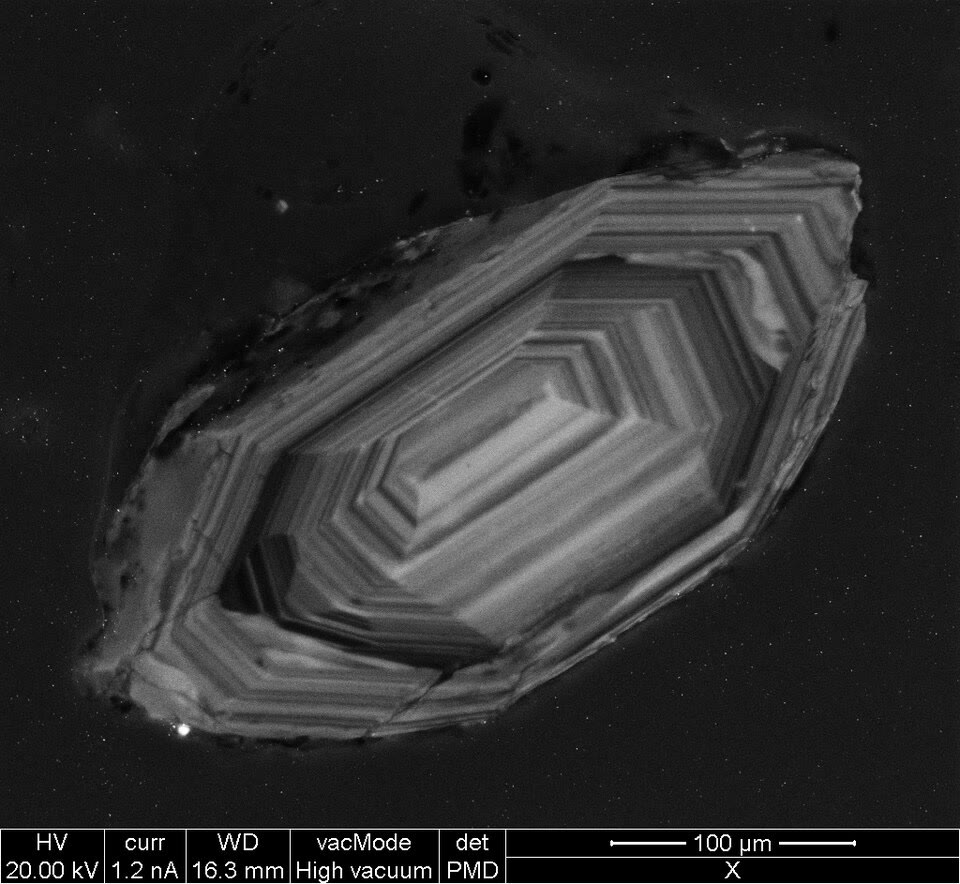
\includegraphics[width=0.5\linewidth]{images/book3/b1-zircon-cl.jpg}

{\small 一颗锆石颗粒，长约三分之一毫米，经
借其在扫描电子显微镜电子束作用下发出的光成像
（阴极发光）。沿晶面分布的条带是
成分略有不同的生长环带，依次形成于
晶体生长过程中。这颗锆石取自一块砂岩，因此它比砂岩更老：
它测定的是其所侵蚀的源岩的年龄。（照片：Emmanuel Roquette, CC~BY-SA~4.0, 经
维基共享资源。）}
\label{fig:b1:radiometric-methods:zircon}
\end{omfigure}
% ledger: commons:zircon-cl

\begin{recall}
物理分册描述了放射性衰变：放射性同位素的原子核
随机衰变，与温度和压强无关，使得
剩余数目 $N$ 在时间 $t$ 后服从 $N = N_0\,e^{-\lambda t}$，其中
$\lambda$ 为衰变常数；半衰期为 $T = \ln 2/\lambda$。同位素
同一元素的同位素质子数相同，中子数
不同；化学分册描述了质谱仪，它按质量对离子进行\omterm{def:b1:clastic-sediments:sorting}{分选}。
在第 2 册、十二年级中，一块与外界未交换母体或子体原子的岩石或\omterm{def:b1:rock-forming-minerals:mineral}{矿物}
即为封闭系统，而
瓦尔登花岗岩的\omterm{def:b1:rock-forming-minerals:mineral}{矿物}投在铷–锶\omterm{def:b1:radiometric-methods:isochron}{等时线}上，给出
3.1 亿年的年龄。黑\omterm{def:b1:rock-forming-minerals:groups}{云母}、白\omterm{def:b1:rock-forming-minerals:groups}{云母}和\omterm{def:b1:rock-forming-minerals:groups}{角闪石}是
\cref{def:b1:rock-forming-minerals:groups}中的\omterm{def:b1:rock-forming-minerals:groups}{云母}与\omterm{def:b1:rock-forming-minerals:groups}{角闪石}。两个已测年层位之间的
年龄可以内插（见\cref{prop:b1:stratigraphic-scale:interpolation}）。
\end{recall}
% ledger: tulane:radiometric, villa22:rb87

\section{衰变体系}\label{sec:b1:radiometric-methods:systems}

一个计时器需要两个计数：母体剩下的量，以及
自计时开始以来子体生成了多少。

\begin{definition}[母同位素，放射成因子体]\label{def:b1:radiometric-methods:radiogenic}
在用于测年的衰变体系中，\emph{母同位素}\index{母同位素}
是指其衰变充当计时器的放射性同位素，而
子体是其衰变产生的同位素。\emph{放射成因
子体}\index{放射成因子体}，记为 $D^*$，是
样品中母体衰变生成的那部分子体，即自计时开始以来
生成的部分；其余部分 $D_0$ 从一开始就存在。今天测得的子体原子数
为 $D = D_0 + D^*$。
\end{definition}

\begin{proposition}[放射成因子体的增长与年龄方程]\label{prop:b1:radiometric-methods:growth}
在一个封闭系统中，若今天含有 $P$ 个母体原子，则\omterm{def:b1:radiometric-methods:radiogenic}{放射成因
子体}在时间 $t$ 内生成的数目为
\[
  D^* = P\,\bigl(e^{\lambda t} - 1\bigr),
\]
假设每次衰变只产生一个子体原子。此时年龄为
\[
  t = \frac{1}{\lambda}\,\ln\!\left(1 + \frac{D^*}{P}\right).
\]
\end{proposition}

\begin{proof}
由衰变律，母体原子数在计时开始时为 $P_0 = P\,e^{\lambda t}$。
在封闭系统中，每个消失的母体原子都变成了一个子体原子，
因此 $D^* = P_0 - P = P\,(e^{\lambda t} - 1)$。于是 $e^{\lambda t} = 1 +
D^*/P$，两边取对数即得年龄。
\end{proof}

年龄只取决于两种原子数之比，这正是质谱仪
最擅长测量的量。下图以半衰期为单位给出两种计数，
经过一个半衰期后 $D^*/P = 1$，经过两个后为 $3$，经过三个后为 $7$
——一般地，比值为 $2^n - 1$ 的时刻，即 $n$ 个半衰期之后。

\begin{omfigure}
\begin{tikzpicture}
\begin{axis}[omrecord, width=0.72\linewidth, height=5.6cm, xmin=0, xmax=5, ymin=0, ymax=1.05,
  xlabel={时间（半衰期）}, ylabel={初始母体的比例},
  xtick={0,1,...,5}, ytick={0,0.25,0.5,0.75,1}]
% computed in figdata/bachelor-1/decay_curves.py (no real-world number)
\addplot[omThm, line width=1pt] table[x=n, y=P] {figdata/out/bachelor-1-decay_curves-curves.dat};
\addplot[omDef, line width=1pt] table[x=n, y=D] {figdata/out/bachelor-1-decay_curves-curves.dat};
\addplot[only marks, mark=*, mark size=1.4pt, black!60] table[x=n, y=P] {figdata/out/bachelor-1-decay_curves-marks.dat};
\addplot[only marks, mark=*, mark size=1.4pt, black!60] table[x=n, y=D] {figdata/out/bachelor-1-decay_curves-marks.dat};
\node[font=\small, text=omThm, anchor=south west] at (axis cs:0.35,0.80) {母体 $P$};
\node[font=\small, text=omDef, anchor=north west] at (axis cs:2.55,0.66) {放射成因子体 $D^*$};
\node[font=\scriptsize, anchor=west, inner sep=1pt] (r1) at (axis cs:0.12,0.5) {$D^*/P = 1$};
\draw[black!60, line width=0.4pt] (r1.east) -- (axis cs:0.95,0.5);
\node[font=\scriptsize, anchor=south] at (axis cs:2,0.77) {$3$};
\node[font=\scriptsize, anchor=south] at (axis cs:3,0.89) {$7$};
\node[font=\scriptsize, anchor=north] at (axis cs:4,0.915) {$15$};
\node[font=\scriptsize, anchor=north east] at (axis cs:4.97,0.95) {$31$};
\end{axis}
\end{tikzpicture}

{\small 封闭系统中母体及其\omterm{def:b1:radiometric-methods:radiogenic}{放射成因子体}，
以占母体初始原子数的分数表示，随以半衰期计量的时间变化。
二者之和始终为一；比值 $D^*/P$ 标于每个整数半衰期处，
每经一个半衰期便加倍再加一。}
\label{fig:b1:radiometric-methods:decay}
\end{omfigure}

时钟只在一定的年龄区间内读数才可靠。在远早于一个半衰期时，
子体只是母体中极小的一部分；经过许多个半衰期后，
剩下的母体过少，难以测量。下表列出最常用的几种体系，
以及各自所适用的测定材料。

\begin{table}[ht]
\centering
\small
\renewcommand{\arraystretch}{1.25}
\begin{tabular}{|l|l|c|c|>{\raggedright\arraybackslash}p{4.3cm}|}
\hline
母体 & 子体 & 半衰期（年） & $\lambda$（每年） & 测年材料 \\
\hline
$^{14}\mathrm{C}$ & $^{14}\mathrm{N}$ & \num{5700} & \num{1.216e-4} & 木材、木炭、骨骼、贝壳 \\
$^{40}\mathrm{K}$ & $^{40}\mathrm{Ar}$，$^{40}\mathrm{Ca}$ & \num{1.25e9} & \num{5.543e-10} & 富钾\omterm{def:b1:rock-forming-minerals:mineral}{矿物}：透\omterm{def:b1:rock-forming-minerals:groups}{长石}、黑\omterm{def:b1:rock-forming-minerals:groups}{云母}、普通\omterm{def:b1:rock-forming-minerals:groups}{角闪石} \\
$^{87}\mathrm{Rb}$ & $^{87}\mathrm{Sr}$ & \num{4.96e10} & \num{1.3972e-11} & 花岗岩（全岩）、\omterm{def:b1:rock-forming-minerals:groups}{云母} \\
$^{147}\mathrm{Sm}$ & $^{143}\mathrm{Nd}$ & \num{1.07e11} & \num{6.46e-12} & 岩石及其\omterm{def:b1:rock-forming-minerals:mineral}{矿物}（\omterm{def:b1:radiometric-methods:isochron}{等时线}） \\
$^{235}\mathrm{U}$ & $^{207}\mathrm{Pb}$ & \num{7.04e8} & \num{9.8485e-10} & 锆石 \\
$^{238}\mathrm{U}$ & $^{206}\mathrm{Pb}$ & \num{4.47e9} & \num{1.55125e-10} & 锆石 \\
\hline
\end{tabular}
\caption{主要衰变体系。钾-40 与两种铀的衰变常数，
为用于计算年龄的约定值；
铷-87 与钐-147 的衰变常数由半衰期算出，
碳-14 的衰变常数则由其半衰期 \num{5700} 年算出。}
\label{tab:b1:radiometric-methods:systems}
\end{table}
% ledger: iaea:c14, iaea:k40-branches, amherst:constants, villa22:rb87, iaea:sm147, iaea:isotopes, tulane:kar, tulane:upb-zircon, tulane:c14

同一原子核有两套数据在使用，年龄值必须注明
所用的是哪一套。核数据表给出钾-40 的半衰期为
\num{1.248e9} 年，并使其衰变中 \qty{10.72}{\percent} 生成氩；
地质年代学中通常采用的常数给出 $\lambda = \num{5.543e-10}$ 每年（半衰期为 \num{1.2505e9}
年），并使 $0.581/5.543 = \qty{10.48}{\percent}$ 的衰变生成氩。
如\cref{sec:b1:radiometric-methods:kar}所述，\omterm{def:b1:radiometric-methods:radiocarbon}{放射性碳年龄}
是用半衰期为 \num{5568} 年的数值计算的，而这一数值已知偏短。两者之差可达百分之几，
远大于目前最佳年龄所给出的 \qty{0.01}{\percent} 精度
（见\cref{sec:b1:radiometric-methods:sediments}）。
钾-40 本身衰变常数的不确定度，它是一个具有两条分支、
半衰期很长的原子核，限制了其年龄的准确度。
% ledger: iaea:k40-branches, amherst:constants, sp77:conventional-age, ics:base.Triassic, nmgrl:arar

\begin{proposition}[年龄的精度]\label{prop:b1:radiometric-methods:precision}
若比值 $R = D^*/P$ 的测量标准不确定度为 $\sigma_R$，
则年龄的不确定度为
\[
  \sigma_t = \frac{\sigma_R}{\lambda\,(1 + R)}.
\]
\end{proposition}

\begin{proof}
对于微小误差 $\delta R$，年龄 $t = \ln(1+R)/\lambda$ 的改变量为
$\delta t = t'(R)\,\delta R = \delta R/\bigl(\lambda(1 + R)\bigr)$.
\end{proof}

对于年轻样品，$R$ 很小，$\sigma_t \approx \sigma_R/\lambda$：
年龄的绝对误差取决于能对少量子体测得多精确，
长半衰期（即较小的 $\lambda$）会将其放大。这也是为什么
铷–锶与铀–铅适用于年龄大于约一千万年的岩石，
而钾–氩可用于年轻至约一万年的岩石，
放射性碳则覆盖最近的 \num{70000} 年。
% ledger: tulane:ranges

\section{等时线}\label{sec:b1:radiometric-methods:isochrons}

年龄方程需要 $D^*$，而仪器测量的是 $D = D_0 + D^*$，
而 $D_0$ 很少为零：凡在形成时吸收过锶的\omterm{def:b1:rock-forming-minerals:mineral}{矿物}中，
均存在锶-87。\omterm{def:b1:radiometric-methods:isochron}{等时线}通过测量若干个起始时子体元素同位素组成相同的样品，
以消除 $D_0$。

\begin{definition}[等时线，初始比值]\label{def:b1:radiometric-methods:isochron}
设 $S$ 为子体元素的一种稳定同位素，它不由任何衰变产生
（对锶为 $^{86}\mathrm{Sr}$，对钕为 $^{144}\mathrm{Nd}$）。
在 $y = D/S$ 对 $x = P/S$ 的图中，落在同一直线上的样品
同时形成，具有相同的 $D/S$ 值，且此后一直为封闭系统；该直线即
称为\emph{等时线}\index{等时线}。这一共同的起始值
$y_0 = (D/S)_0$ 即为\emph{初始比值}\index{初始比值}。
\end{definition}
% ledger: tulane:radiometric, tulane:c14

\begin{theorem}[等时线]\label{thm:b1:radiometric-methods:isochron}
同时形成、具有相同\omterm{def:b1:radiometric-methods:isochron}{初始比值} $y_0$，且已作为封闭系统经历时间 $t$ 的样品，
满足
\[
  y = y_0 + \bigl(e^{\lambda t} - 1\bigr)\,x .
\]
其点位于斜率为 $m = e^{\lambda t} - 1$、截距为 $y_0$ 的直线上，
且 $t = \ln(1+m)/\lambda$。
\end{theorem}

\begin{proof}
对每个样品，由 $D = D_0 + P\,(e^{\lambda t} - 1)$ 及
\cref{prop:b1:radiometric-methods:growth}，$S$ 的原子数未变，因为 $S$ 稳定、不由任何衰变产生，且体系封闭；
以其除之，即得 $y = y_0 + (e^{\lambda t} - 1)\,x$，
其中 $y_0$ 对各样品相同，
依假设。
\end{proof}

当花岗岩结晶时，其所有样品具有相同的 $y_0$，在图上位于一条水平线上；
此后每个样品都按其 $x$ 的比例上移，而直线
绕其截距转动。样品需要不同的 $x$ 值，才能把斜率定好：
如第 2 册所述，可取含铷多与含铷少的\omterm{def:b1:rock-forming-minerals:mineral}{矿物}，或
取自同一侵入体中分异程度不同部分的全岩样品。
偏离直线的点，表明该样品并非封闭系统，或其未共享相同的
\omterm{def:b1:radiometric-methods:isochron}{初始比值}。\omterm{def:b1:radiometric-methods:isochron}{初始比值}本身即是一种示踪剂：源自\omterm{def:b1:layered-earth:layers}{地幔}的岩浆
继承了较低的 $^{87}\mathrm{Sr}/^{86}\mathrm{Sr}$，约为 $0.7025$，而来自熔融大陆\omterm{def:b1:layered-earth:layers}{地壳}的岩浆
则具有较高的值，约为 $0.710$，这是因为\omterm{def:b1:layered-earth:layers}{地壳}富含
铷，并在漫长的地质历史中生成了更多的锶-87。
% ledger: tulane:radiometric, tulane:sr-initial

实测点从来不会恰好落在一条直线上。通常对直线的估计，是
使各点到直线的竖直距离平方和
尽可能小的那一条。

\begin{proposition}[最小二乘直线]\label{prop:b1:radiometric-methods:lsq}
设 $(x_i, y_i)$，$i = 1, \dots, n$，为若干点，其中至少有两个不同的 $x_i$，
其均值分别为 $\bar x$ 与 $\bar y$，并令
\[
  S_{xx} = \sum_i (x_i - \bar x)^2, \qquad S_{xy} = \sum_i (x_i - \bar x)(y_i - \bar y).
\]
直线 $y = b + m x$ 使 $Q(b, m) = \sum_i (y_i - b - m x_i)^2$ 最小，其系数为
\[
  m = \frac{S_{xy}}{S_{xx}}, \qquad b = \bar y - m\,\bar x ,
\]
且过质心 $(\bar x, \bar y)$。
\end{proposition}

\begin{proof}
$Q$ 是平方和，即关于 $(b, m)$ 的二次多项式，在各方向上都趋于
无穷大，故函数在两个偏导数
同时为零处取得最小值：$\partial Q/\partial b = -2 \sum_i (y_i - b - m x_i) = 0$。
由此得 $n\bar y = n b + n m \bar x$，于是 $b = \bar y - m \bar x$，直线
经过质心。代入，$y_i - b - m x_i = (y_i - \bar y) - m(x_i -
\bar x)$，且 $\partial Q/\partial m = -2 \sum_i x_i \bigl[(y_i - \bar y) - m(x_i
- \bar x)\bigr] = 0$。由于 $\sum_i (y_i - \bar y) = \sum_i (x_i - \bar x) = 0$，$x_i$
可替换为 $x_i - \bar x$ 代入此和式，得 $S_{xy} - m S_{xx} = 0$。
$S_{xx} > 0$，因各 $x_i$ 不全相等。
\end{proof}

各点围绕直线的散布决定了斜率的不确定度。
记残差 $r_i = y_i - b - m x_i$，则散布的标准差
为 $s = \sqrt{\sum_i r_i^2/(n-2)}$——两个参数占用两个自由度——
斜率与
截距的标准不确定度分别为
\[
  \sigma_m = \frac{s}{\sqrt{S_{xx}}}, \qquad
  \sigma_b = s\,\sqrt{\frac1n + \frac{\bar x^2}{S_{xx}}} .
\]
这两个统计结果在本阶段不加证明地承认；年龄的
不确定度为 $\sigma_t = \sigma_m/\bigl(\lambda(1 + m)\bigr)$，
由\cref{prop:b1:radiometric-methods:precision}的论证得出。它们说明好的\omterm{def:b1:radiometric-methods:isochron}{等时线}需要：
数据点多，$x$ 分布广（$S_{xx}$ 大），
散布小。

\begin{method}[拟合等时线]\label{met:b1:radiometric-methods:isochron}
\begin{enumerate}
  \item 在同一天体的至少四个样品中测量 $x = P/S$ 与 $y = D/S$，
        样品应选取为使 $x$ 尽可能分散。
  \item 作图；凡明显偏离趋势的点，须说明理由后舍去。
  \item 计算 $\bar x$、$\bar y$、$S_{xx}$、$S_{xy}$，再算 $m = S_{xy}/S_{xx}$
        及 $b = \bar y - m \bar x$。
  \item 计算残差、$s$、$\sigma_m$ 与 $\sigma_b$。
  \item 年龄为 $t = \ln(1+m)/\lambda$，其中 $\sigma_t =
        \sigma_m/\bigl(\lambda(1+m)\bigr)$；\omterm{def:b1:radiometric-methods:isochron}{初始比值}为 $b \pm \sigma_b$。
\end{enumerate}
\end{method}

\begin{example}[一个虚构的流纹岩]\label{ex:b1:radiometric-methods:rhyolite}
取一系列流纹岩熔岩的六个全岩样品（练习数据），结果如下：
\begin{center}
\small
\begin{tabular}{|l|cccccc|}
\hline
$x = {}^{87}\mathrm{Rb}/^{86}\mathrm{Sr}$ & 1.85 & 4.62 & 9.30 & 14.75 & 21.20 & 27.60 \\
$y = {}^{87}\mathrm{Sr}/^{86}\mathrm{Sr}$ & 0.71732 & 0.73332 & 0.76164 & 0.79420 & 0.83226 & 0.87028 \\
\hline
\end{tabular}
\end{center}
此处 $\bar x = 13.22$，$\bar y = 0.784837$，$S_{xx} = 491.41$，
$S_{xy} = 2.92308$，于是 $m = 0.0059484$，$b = 0.70620$。残差给出
$s = 0.00024$，$\sigma_m = \num{1.10e-5}$，$\sigma_b = 0.00018$。年龄为
$t = \ln(1.0059484)/\num{1.3972e-11} = \qty{424.5}{\Ma}$，其
不确定度为 $\sigma_t = \num{1.10e-5}/(\num{1.3972e-11} \times 1.0059) = \qty{0.8}{\Ma}$：
\qty[uncertainty-mode=separate]{424.5(8)}{\Ma}，\omterm{def:b1:radiometric-methods:isochron}{初始比值}
\num[uncertainty-mode=separate]{0.70620(18)}（见下图）。
\end{example}
% values: isochron.py (slope 0.005948361, intercept 0.7061993, age 424.4732, sigma 0.7827871); ledger: villa22:rb87

\begin{omfigure}
\begin{tikzpicture}
\begin{axis}[omrecord, width=0.74\linewidth, height=6cm, xmin=0, xmax=30, ymin=0.70, ymax=0.88,
  xlabel={$^{87}\mathrm{Rb}/^{86}\mathrm{Sr}$}, ylabel={$^{87}\mathrm{Sr}/^{86}\mathrm{Sr}$},
  ytick={0.70,0.72,...,0.88},
  y tick label style={/pgf/number format/.cd, fixed, fixed zerofill, precision=2}]
% computed in figdata/bachelor-1/isochron.py (exercise data, invented rhyolite); ledger: villa22:rb87
\addplot[black!60, densely dotted, line width=0.7pt] table[x=x, y=y] {figdata/out/bachelor-1-isochron-initial.dat};
\addplot[omDef, line width=0.9pt] table[x=x, y=y] {figdata/out/bachelor-1-isochron-line.dat};
\addplot[omThm, only marks, mark=*, mark size=2pt] table[x=x, y=y] {figdata/out/bachelor-1-isochron-points.dat};
\node[font=\scriptsize, text=omDef, anchor=south east, align=right] at (axis cs:19,0.83)
  {最小二乘斜率 $0.005948$\\ 年龄 \qty[uncertainty-mode=separate]{424.5(8)}{\Ma}};
\node[font=\scriptsize, text=black!70, anchor=south west] at (axis cs:9,0.7068)
  {初始比值 $0.70620$，为熔岩形成时};
\end{axis}
\end{tikzpicture}

{\small 虚构流纹岩六个全岩样品的铷–锶\omterm{def:b1:radiometric-methods:isochron}{等时线}（练习数据）。
数据点围绕最小二乘直线略有散布。
该直线过数据点的质心；虚线为所有点
在熔岩形成时的位置。}
\label{fig:b1:radiometric-methods:isochron}
\end{omfigure}

\begin{inthelab}[称量同位素]
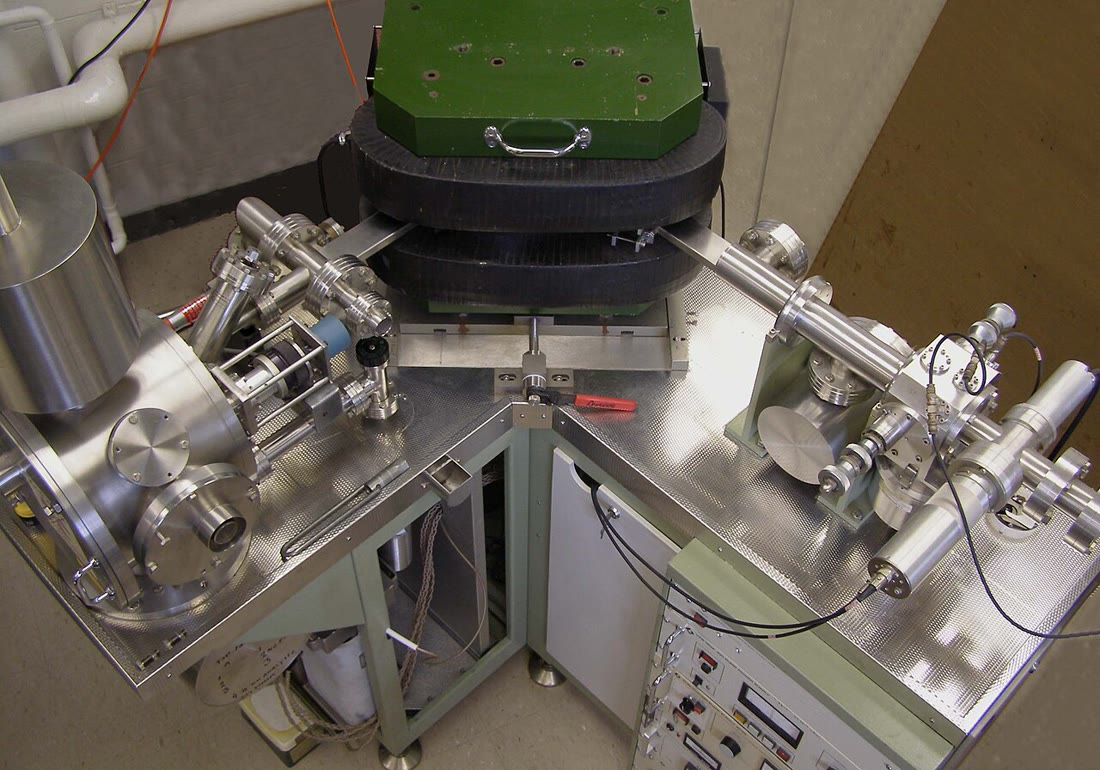
\includegraphics[width=0.42\linewidth]{images/book3/b1-tims.jpg}\hfill
\begin{minipage}[b]{0.55\linewidth}
热电离质谱仪（左图）用于测量同位素比值，
如锶等元素。待测元素由溶解的样品经
化学分离后，装在真空中的金属灯丝上，加热后释出离子，
离子在大型电磁铁（
中央的黑色线圈）的磁场中加速并偏转，轻离子偏转更多，重离子偏转较少，使每种
同位素各自到达对应的收集器。仪器最擅长测量的是同位素比值，
这也正是基于比值的方法最精确的原因。
（照片：Radiogenic，CC0，经维基共享资源。）
\end{minipage}
\end{inthelab}
% ledger: commons:tims, amherst:constants

\section{钾–氩、铀–铅与放射性碳}\label{sec:b1:radiometric-methods:kar}

\subsection*{一个母体与两个子体}

\begin{definition}[分支衰变]\label{def:b1:radiometric-methods:branching}
当母体原子核经两条或更多途径衰变为不同子体时，称母体发生\emph{分支衰变}\index{分支衰变}。
每条途径 $i$ 各有其
分衰变常数 $\lambda_i$，母体以总衰变常数
$\lambda = \sum_i \lambda_i$，其中占比 $\lambda_i/\lambda$ 的衰变
走途径~$i$。钾-40 衰变为钙-40 时，$\lambda_\beta =
\num{4.962e-10}$ 每年；衰变为氩-40 时，$\lambda_e = \num{0.581e-10}$ 每
年。
\end{definition}
% ledger: amherst:constants, iaea:k40-branches

\begin{proposition}[钾–氩年龄]\label{prop:b1:radiometric-methods:kar}
某\omterm{def:b1:rock-forming-minerals:mineral}{矿物}保留了其中生成的全部氩，且形成时不含氩，
经过时间 $t$ 后，其中含有
\[
  {}^{40}\mathrm{Ar}^* = \frac{\lambda_e}{\lambda}\;{}^{40}\mathrm{K}\,\bigl(e^{\lambda t} - 1\bigr),
  \qquad\text{则}\qquad
  t = \frac{1}{\lambda}\,\ln\!\left(1 + \frac{\lambda}{\lambda_e}\,
      \frac{{}^{40}\mathrm{Ar}^*}{{}^{40}\mathrm{K}}\right),
\]
其中 ${}^{40}\mathrm{K}$ 为今日钾-40 原子数，且 $\lambda =
\lambda_\beta + \lambda_e$。
\end{proposition}

\begin{proof}
母体以总常数 $\lambda$ 衰变，与途径无关，
由\cref{prop:b1:radiometric-methods:growth}可知，时间 $t$ 内的衰变数为
${}^{40}\mathrm{K}\,(e^{\lambda t} - 1)$。每次衰变走氩途径的概率为
$\lambda_e/\lambda$，各次衰变相互独立；在极大量的
衰变次数中，产生氩的比例为 $\lambda_e/\lambda$。
由此得 ${}^{40}\mathrm{Ar}^*$；解出 $t$ 即得年龄。
\end{proof}

指数中用的是总衰变常数，前面的系数用的是分衰变常数：
若在指数中用 $\lambda_e$，仿佛氩是唯一途径，
会得出严重失真的年龄。钙分支承担了十分之九的衰变，却
对定年毫无用处，因为钙-40 是一种
在岩石中丰富的元素的常见同位素；氩为稀有气体，会从熔体中逸出，因此晶体
形成时几乎不含氩。钾-40 占钾原子的
\qty{0.0117}{\percent}。钾与氩的绝对含量须分别测定。
来自空气的氩存在于每块岩石中，可借氩-36 识别，
并用大气比值
$^{40}\mathrm{Ar}/^{36}\mathrm{Ar} = 295.5$ 予以扣除。
% ledger: tulane:kar, iaea:k40-branches, amherst:constants, nmgrl:kar

该方法有两种失效方式。过剩氩使年龄偏老：冷却迅速的熔岩
可能将来自\omterm{def:b1:layered-earth:layers}{地幔}的氩包裹于气泡中，而历史熔岩
通常给出 100 万至 200 万年的钾–氩年龄，这一误差
只对年轻岩石才有影响。氩的丢失使年龄偏年轻：多数\omterm{def:b1:rock-forming-minerals:mineral}{矿物}
加热到约 \qty{300}{\celsius} 以上时会失去氩，因此后来的
变质作用会全部或部分重置计时；部分丢失则得到一个
介于两次事件之间的年龄，不代表任何一次事件。富钾\omterm{def:b1:rock-forming-minerals:mineral}{矿物}
较为优先：透\omterm{def:b1:rock-forming-minerals:groups}{长石}与黑\omterm{def:b1:rock-forming-minerals:groups}{云母}，其次为\omterm{def:b1:rock-forming-minerals:groups}{斜长石}或\omterm{def:b1:rock-forming-minerals:groups}{角闪石}。
% ledger: tulane:kar, nmgrl:kar

氩–氩法只测量比值。样品在核反应堆堆芯中受快中子照射，
与一块已知年龄的标准\omterm{def:b1:rock-forming-minerals:mineral}{矿物}并排放置；
反应使其中一部分钾-39 转变为氩-39，后者
代表钾的含量，标准\omterm{def:b1:rock-forming-minerals:mineral}{矿物}则给出反应的产率。
两种同位素在同一气体中一并测量。样品随后可
分步加热，可用熔炉或激光器；每一步给出一个年龄，
各年龄对释放的氩-39 累积比例作图，构成
年龄谱。误差范围内彼此一致的各步构成一个坪；无坪的谱
则警示\omterm{def:b1:rock-forming-minerals:mineral}{矿物}未能保持封闭。撞击与白垩纪末
灭绝之间的同步性，依据的是
氩–氩年龄。
% ledger: amherst:arar, nmgrl:arar, renne:kpg

\subsection*{两个铀钟}

铀有两种长寿命同位素：铀-238 衰变为铅-206，
铀-235 衰变为铅-207，二者速率不同；今天
$^{235}\mathrm{U}/^{238}\mathrm{U} = 0.0072567$，即每 137.8 个原子中有一个。
含铀\omterm{def:b1:rock-forming-minerals:mineral}{矿物}因此携带两个独立的铀钟，各有
自身的生长方程，${}^{206}\mathrm{Pb}^* = {}^{238}\mathrm{U}\,(e^{\lambda_{238} t} - 1)$
以及 ${}^{207}\mathrm{Pb}^* = {}^{235}\mathrm{U}\,(e^{\lambda_{235} t} - 1)$。若两个
年龄一致，则称二者协和，这种一致是检验
\omterm{def:b1:rock-forming-minerals:mineral}{矿物}保持封闭的检验，这是单个时钟无法提供的。不一致
主要来自晶体中被铀自身辐射破坏的部分所丢失的铅；
将两个比值相互作图，
即协和图，可同时恢复晶体的年龄，
以及使其丢失铅的事件的年龄——这是本科三年级分册中的一种工具。
% ledger: amherst:constants, tulane:upb-zircon

锆石，$\mathrm{ZrSiO_4}$，是首选\omterm{def:b1:rock-forming-minerals:mineral}{矿物}：它能将铀纳入
晶体结构，却几乎不容纳铅，因此其中几乎所有的铅都是放射成因的；它
坚硬，抗风化，能经受变质作用，因此由岩石侵蚀而来的颗粒
在由其衍生的沙中仍保留其年龄。磷灰石与榍石也
有应用，但较少。
% ledger: tulane:upb-zircon, commons:zircon-cl

\subsection*{放射性碳}

碳-14 在高层大气中不断生成，由被宇宙射线
轰击的氮-14 生成。它并入大气中的碳；生物
与大气交换碳，并保持其中碳-14 的比例。死亡时
交换停止，碳-14 衰变回氮-14。由于初始
比例即大气的比例，年龄仅由衰变定律得出，
无需\omterm{def:b1:radiometric-methods:isochron}{等时线}：$t = -\tau \ln(A/A_0)$，其中 $A$ 为
样品碳的活度，$A_0$ 为活体碳的活度，$\tau =
1/\lambda$ 为平均寿命。木材、木炭、骨骼、牙齿和贝壳均以此法测年，
可追溯至数万年，至多约 \num{70000} 年。
% ledger: tulane:c14, iaea:c14

\begin{definition}[放射性碳年龄、标准曲线]\label{def:b1:radiometric-methods:radiocarbon}
样品的（常规）\emph{放射性碳年龄}\index{放射性碳年龄}为
\[
  t = -8033 \,\ln \frac{A_{\mathrm{SN}}}{A_{\mathrm{ON}}} \ \text{年 BP},
\]
其中 $A_{\mathrm{SN}}$ 为样品碳的活度，
$A_{\mathrm{ON}}$ 为参考标准的活度；采用半衰期
为 \num{5568} 年（平均寿命 \num{8033} 年），对活度作归一化，
以校正碳的同位素分馏（$\delta^{13}\mathrm{C} = \qty{-25}{\permil}$），
并以公元 1950 年以前的年数计年（BP，“现在之前”）。一条
\emph{标准曲线}\index{标准曲线}给出已知日历年龄样品的放射性碳年龄；
反过来用时，它可把放射性碳年龄换算为
一段日历年龄范围（cal BP）。
\end{definition}
% ledger: sp77:conventional-age, reimer20:intcal20

\omterm{def:b1:radiometric-methods:radiocarbon}{放射性碳年龄}并非日历年龄，原因有两点。其一，
Libby 所取、按惯例沿用的半衰期为 \num{5568} 年，比真实的 \num{5700} 年短，因此\omterm{def:b1:radiometric-methods:radiocarbon}{放射性碳年龄}大约
偏小 \qty{2.4}{\percent}。更重要的是，大气中碳-14 的
比例并不恒定。\omterm{def:b1:radiometric-methods:radiocarbon}{标准曲线}同时测定这两种效应，
所用档案均已独立定年：树轮可追溯至约
\num{13900} cal BP，更早的则包括漂浮树轮序列、湖泊与海洋沉积物、洞穴沉积物及珊瑚，
直至 \num{55000} cal BP（见下图）。
% ledger: sp77:conventional-age, iaea:c14, reimer20:intcal20

\begin{omfigure}
\begin{tikzpicture}
\begin{axis}[name=main, omrecord, width=0.5\linewidth, height=6cm, xmin=0, xmax=12, ymin=0, ymax=12,
  xlabel={日历年龄（千 cal BP）}, ylabel={放射性碳年龄（千 BP）},
  xtick={0,2,...,12}, ytick={0,2,...,12}]
% figdata/bachelor-1/radiocarbon.py, IntCal20 (dataset bachelor-1-intcal20); ledger: data:b3-intcal20
\addplot[black!50, dashed, domain=0:12, samples=2] {x};
\addplot[omDef, line width=0.9pt] table[x=cal, y=c14] {figdata/out/bachelor-1-radiocarbon-curve.dat};
\draw[omThm, line width=0.6pt] (axis cs:2.3,2.3) rectangle (axis cs:2.9,2.9);
\node[font=\scriptsize, anchor=east, text=black!60] at (axis cs:8.4,10.4) {等年龄线};
\node[font=\scriptsize, text=omDef, anchor=north west] at (axis cs:7.4,5.6) {标准曲线};
\end{axis}
\begin{axis}[at={(main.east)}, anchor=west, xshift=2.1cm, omrecord, width=0.38\linewidth, height=6cm,
  xmin=2300, xmax=2900, ymin=2300, ymax=2900, xlabel={日历年龄（cal BP）}, ylabel={放射性碳年龄（BP）},
  xtick={2300,2500,2700,2900}, ytick={2300,2500,2700,2900},
  x tick label style={/pgf/number format/.cd, set thousands separator={}},
  y tick label style={/pgf/number format/.cd, set thousands separator={}}]
\addplot[name path=hi, draw=none, forget plot] table[x=cal, y=hi] {figdata/out/bachelor-1-radiocarbon-zoom.dat};
\addplot[name path=lo, draw=none, forget plot] table[x=cal, y=lo] {figdata/out/bachelor-1-radiocarbon-zoom.dat};
\addplot[omDef!25, forget plot] fill between[of=hi and lo];
\addplot[omDef, line width=0.8pt] table[x=cal, y=c14] {figdata/out/bachelor-1-radiocarbon-zoom.dat};
\addplot[omThm, line width=0.6pt, domain=2300:2900, samples=2] {2480};
\draw[omThm, densely dotted] (axis cs:2495,2300) -- (axis cs:2495,2480);
\draw[omThm, densely dotted] (axis cs:2699,2300) -- (axis cs:2699,2480);
\node[font=\scriptsize, text=omThm, anchor=south west] at (axis cs:2310,2485) {$2480$ BP};
\end{axis}
\end{tikzpicture}

{\small 左：过去 \num{12000} 年的 IntCal20 \omterm{def:b1:radiometric-methods:radiocarbon}{标准曲线}，
纵轴为\omterm{def:b1:radiometric-methods:radiocarbon}{放射性碳年龄}、横轴为日历年龄；虚线为两者相等之处。
右：放大左图中的方框，并画出曲线一个标准不确定度的带宽。
在 \num{2500} 至 \num{2700} cal BP 之间曲线近乎平坦：
\omterm{def:b1:radiometric-methods:radiocarbon}{放射性碳年龄} 2480 年 BP 对应的日历年龄约为
\num{2495} 至 \num{2699} cal BP。}
\label{fig:b1:radiometric-methods:intcal}
\end{omfigure}
% ledger: data:b3-intcal20, reimer20:intcal20

在 \num{2000} cal BP 处，\omterm{def:b1:radiometric-methods:radiocarbon}{标准曲线}给出 \num[uncertainty-mode=separate]{2070 \pm 14} 年 BP；在
\num{12000} cal BP 处，为 \num{10306}：该处\omterm{def:b1:radiometric-methods:radiocarbon}{放射性碳年龄}比日历年龄小 \num{1694} 年，
远大于半衰期所对应的 \qty{2.4}{\percent}。
曲线有起伏，在其平坦处，
无论测量多么精确，一个\omterm{def:b1:radiometric-methods:radiocarbon}{放射性碳年龄}都会对应一段较长的日历年龄范围。
% ledger: data:b3-intcal20

\begin{dated}{2020}
% ledger: reimer20:intcal20
北半球通用的\omterm{def:b1:radiometric-methods:radiocarbon}{标准曲线}为 IntCal20，发表于 2020 年。它
取代了 IntCal13，增加了新数据，并将曲线延伸至 \num{55000} cal BP，
同时为南半球和表层海洋分别给出了独立的曲线。
\omterm{def:b1:radiometric-methods:radiocarbon}{标准曲线}会随着新档案的测定而修订，因此一个日历年龄
必须注明产生它的曲线。
\end{dated}

\section{闭合温度}\label{sec:b1:radiometric-methods:closure}

从岩浆中结晶的\omterm{def:b1:rock-forming-minerals:mineral}{矿物}，形成时温度为 \qty{800}{\celsius}，
其计时也不会立即开始。在高温时，子体原子——尤其是氩——
会穿过其晶格扩散并逸出；只有当\omterm{def:b1:rock-forming-minerals:mineral}{矿物}充分冷却后，
扩散才慢到可以忽略，子体开始积累。
% ledger: leeds:closure, tulane:kar, tulane:magma-types

\begin{definition}[闭合温度，冷却年龄]\label{def:b1:radiometric-methods:closure}
对某一衰变体系，\omterm{def:b1:rock-forming-minerals:mineral}{矿物}的\emph{闭合温度}\index{闭合温度}
是这样一个温度：低于此温度时，母体与子体原子
进出其晶格的扩散已慢到可以忽略，使\omterm{def:b1:rock-forming-minerals:mineral}{矿物}表现为封闭系统。
\emph{冷却年龄}\index{冷却年龄}是在闭合温度以上形成的\omterm{def:b1:rock-forming-minerals:mineral}{矿物}中测得的
年龄，它给出的是\omterm{def:b1:rock-forming-minerals:mineral}{矿物}冷却穿过该温度的时刻，
而非其形成的
时刻。
\end{definition}
% ledger: leeds:closure

\omterm{def:b1:radiometric-methods:closure}{闭合温度}因\omterm{def:b1:rock-forming-minerals:mineral}{矿物}而异，因为晶格不同；也因元素而异，
因为不同原子在同一晶格中的扩散速率不同
（见下图）。这些数值只是近似的：两份表格给出黑\omterm{def:b1:rock-forming-minerals:groups}{云母}中氩的\omterm{def:b1:radiometric-methods:closure}{闭合温度}分别为 \qty{280}{\celsius} 和
\qty{350}{\celsius}，\omterm{def:b1:rock-forming-minerals:groups}{角闪石}中氩的则为 \qty{530}{\celsius} 和
\qty{550}{\celsius}。裂变径迹，即晶体中
因铀核自发裂变而留下的损伤痕迹，在更低的温度下
即会愈合。
% ledger: leeds:closure, amherst:closure

\begin{omfigure}
\begin{tikzpicture}
\begin{axis}[width=0.8\linewidth, height=7cm, xbar, bar width=7pt, xmin=0, xmax=850,
  xlabel={闭合温度（\unit{\celsius}）},
  symbolic y coords={zrupb,spupb,hbar,mssr,msar,btsr,btar,zrft,kfsar,apft},
  ytick={zrupb,spupb,hbar,mssr,msar,btsr,btar,zrft,kfsar,apft}, y dir=reverse, enlarge y limits=0.07,
  yticklabels={{锆石，U--Pb},{榍石，U--Pb},{角闪石，K--Ar},{白云母，Rb--Sr},{白云母，K--Ar},{黑云母，Rb--Sr},{黑云母，K--Ar},{锆石，裂变径迹},{钾长石，K--Ar},{磷灰石，裂变径迹}},
  y tick label style={font=\scriptsize}, x tick label style={font=\scriptsize},
  axis x line*=bottom, axis y line*=left]
% ledger: leeds:closure (values as tabulated; > lower bound, ~ approximate, ranges and +- as given)
\addplot[fill=omDef!55, draw=omDef, error bars/.cd, x dir=both, x explicit]
  coordinates {(750,zrupb) (650,spupb) (530,hbar) +- (40,0) (500,mssr) (350,msar) (320,btsr)
               (280,btar) +- (40,0) (200,zrft) +- (25,0) (130,kfsar) (105,apft) +- (10,0)};
\node[font=\scriptsize, anchor=west] at (axis cs:755,zrupb) {$> 750$};
\node[font=\scriptsize, anchor=west] at (axis cs:655,spupb) {$> 650$};
\node[font=\scriptsize, anchor=west] at (axis cs:575,hbar) {$530 \pm 40$};
\node[font=\scriptsize, anchor=west] at (axis cs:505,mssr) {$500$};
\node[font=\scriptsize, anchor=west] at (axis cs:355,msar) {$\approx 350$};
\node[font=\scriptsize, anchor=west] at (axis cs:325,btsr) {$320$};
\node[font=\scriptsize, anchor=west] at (axis cs:325,btar) {$280 \pm 40$};
\node[font=\scriptsize, anchor=west] at (axis cs:230,zrft) {$175$--$225$};
\node[font=\scriptsize, anchor=west] at (axis cs:135,kfsar) {$\approx 130$，有漏失};
\node[font=\scriptsize, anchor=west] at (axis cs:120,apft) {$105 \pm 10$};
\end{axis}
\end{tikzpicture}

{\small 主要\omterm{def:b1:rock-forming-minerals:mineral}{矿物}时钟的封闭温度，取自一份已发表的表格。
U--Pb 为铀–铅，K--Ar 为钾–氩（及氩–氩），Rb--Sr
为铷–锶。对于裂变径迹，该值为径迹
愈合时的温度。}
\label{fig:b1:radiometric-methods:closure}
\end{omfigure}

在缓慢冷却的深成岩体中，各时钟因此依次关闭，
从最热到最冷：锆石最先关闭，接近其结晶时，随后是
\omterm{def:b1:rock-forming-minerals:groups}{角闪石}，再之后是白\omterm{def:b1:rock-forming-minerals:groups}{云母}和黑\omterm{def:b1:rock-forming-minerals:groups}{云母}。它们年龄的差异记录了
冷却过程。

\begin{proposition}[两次封闭之间的冷却速率]\label{prop:b1:radiometric-methods:cooling}
若同一岩石的两种\omterm{def:b1:rock-forming-minerals:mineral}{矿物}，封闭温度为 $T_1 > T_2$，
其\omterm{def:b1:radiometric-methods:closure}{冷却年龄}为 $t_1 > t_2$，则两次封闭之间的平均冷却速率为
\[
  \dot T = \frac{T_1 - T_2}{t_1 - t_2}.
\]
若岩石位于一个深度，该处温度随深度以恒定梯度 $G$ 升高，
地表温度为 $T_s$，岩石所处深度为 $z_i
= (T_i - T_s)/G$，即时钟 $i$ 关闭时的深度。
\end{proposition}

\begin{proof}
岩石温度为 $T_1$ 时对应时间 $t_1$，温度为 $T_2$ 时对应时间 $t_2$；其温度的平均变化率
为两者差值之比。在
线性\omterm{def:b1:heat-budget:geotherm}{地温线}（\cref{def:b1:heat-budget:geotherm}）下，$T = T_s + G z$，由此
即可得出深度。
\end{proof}

深度可给出折返速率，前提是岩石抵达地表的时间
已知——如本章的问题所示。该方法较粗略：
封闭温度的不确定度达数十摄氏度，且\omterm{def:b1:heat-budget:geotherm}{地温线}
假定随时间保持不变。热年代学，
即利用众多时钟对温度–时间路径进行的精细重建，
是本科三年级分册的内容。

\section{沉积序列的定年}\label{sec:b1:radiometric-methods:sediments}

大多数沉积岩无法直接定年，因为其颗粒比岩石本身更老，
如本章开头那颗碎屑锆石：它给出的是
被剥蚀母岩的年龄。放射性碳只能测定年轻的有机物。因此，图中的年龄
来自那些在沉积时刻即已结晶的岩石，
即序列中的火山灰层和熔岩流，
以及切穿该序列的火成岩。
% ledger: tulane:upb-zircon, tulane:c14, commons:zircon-cl

\begin{definition}[限定年龄]\label{def:b1:radiometric-methods:bracketing}
称\emph{限定年龄}\index{限定年龄}为对某沉积层年龄施加的一种限制，
该限制由依地层学原理与之相关的已定年岩石给出：
地层学原理：由其下方某已定年层或其中最年轻的
碎屑颗粒给出的最大年龄；由其上方某已定年层，或切穿它的
侵入体给出的最小年龄。介于最大与最小年龄之间的层位即被限定。
\end{definition}

\begin{omfigure}
\begin{tikzpicture}[x=1cm, y=0.62cm]
  % column
  \fill[lith shale] (0,0) rectangle (2.4,3);
  \fill[lith sandstone] (0,3) rectangle (2.4,6);
  \fill[lith shale] (0,6) rectangle (2.4,9);
  \fill[lith limestone] (0,9) rectangle (2.4,12);
  \draw (0,0) rectangle (2.4,12);
  % ash bed below, lava flow above
  \fill[omThm!70] (0,2.0) rectangle (2.4,2.3);
  \fill[black!65] (0,9.0) rectangle (2.4,9.6);
  % boundary
  \draw[omDef, line width=1.2pt] (-0.3,7.2) -- (2.7,7.2);
  % dyke cutting everything
  \fill[black!40] (1.55,0) -- (1.85,0) -- (1.95,12) -- (1.65,12) -- cycle;
  % detrital zircons
  \foreach \p in {(0.4,3.6),(0.9,4.5),(0.5,5.4),(1.2,3.9),(0.8,5.0)}
    \fill[omThm] \p circle (1.3pt);
  % labels
  \node[anchor=west, font=\small, align=left] at (3.0,2.15) {火山灰层，$t_1$：最大年龄};
  \node[anchor=west, font=\small, align=left] at (3.0,4.5) {最年轻碎屑锆石，$t_0$：\\砂岩的最大年龄};
  \node[anchor=west, font=\small, text=omDef] at (3.0,7.2) {待定年层};
  \node[anchor=west, font=\small, align=left] at (3.0,9.3) {熔岩流，$t_2$：最小年龄};
  \node[anchor=west, font=\small, align=left] at (3.0,11.3) {岩墙，$t_3$：所切穿 \\各层的最小年龄};
  \draw[black!50] (2.5,2.15) -- (2.95,2.15);
  \draw[black!50] (1.25,4.5) -- (2.95,4.5);
  \draw[black!50] (2.5,9.3) -- (2.95,9.3);
  \draw[black!50] (1.95,11.3) -- (2.95,11.3);
\end{tikzpicture}

{\small 限定沉积序列中某一层位的年龄（示意）。
下方的火山灰层与砂岩中最年轻的碎屑锆石给出最大年龄；
上方的熔岩流与切穿整个序列的岩墙给出最小年龄。
该层位比 $t_1$ 年轻，比 $t_2$ 古老；岩墙只说明
它比 $t_3$ 古老。}
\label{fig:b1:radiometric-methods:bracketing}
\end{omfigure}

最好的限定既紧密又精确：两层相距数米的火山灰层，
以锆石定年，精度达数万年，两者之间的层位
由\cref{prop:b1:stratigraphic-scale:interpolation}内插。在煤山，
三叠系底界的 GSSP 位于五层已定年的火山灰层之中；
灭绝事件限定在 \qty[uncertainty-mode=separate]{251.941(37)}{\Ma}
与 \qty[uncertainty-mode=separate]{251.880(31)}{\Ma} 之间，该系底界
定于 \qty[uncertainty-mode=separate]{251.902(24)}{\Ma}
（\cref{sec:b1:stratigraphic-scale:extinctions}）。火山灰层被风
带越相带搬运，既是时间线，也是时钟。
% ledger: burgess:end-permian, gssp:induan, ics:base.Triassic

年代表的精度仅取决于各界线附近的已定年层。三叠系底界
精确到 \qty{0.024}{\Ma}，相对精度为万分之一；石炭系底界
精确到 \qty{0.19}{\Ma}；泥盆系底界
精确到 \qty{1.36}{\Ma}。在界线附近无已定年层处，其年龄
由较远的两层之间内插，不确定度也随之增大。每一
在界线附近新测定年龄的火山灰层都可能使其移动，这正是年代表
附有版本日期的原因。
% ledger: ics:base.Triassic, ics:base.Carboniferous, gssp:lochkovian

\section{练习}

\begin{exercise}[$\star$]\label{exo:b1:radiometric-methods:1}
(a)~某\omterm{def:b1:rock-forming-minerals:mineral}{矿物}中\omterm{def:b1:radiometric-methods:radiogenic}{放射成因子体}原子数为母原子数的三倍。
它的年龄为多少个半衰期？(b)~计算 $D^*/P$ 在
\qty{310}{\Ma} 时的值，分别对铷-87 与铀-235，并采用
\cref{tab:b1:radiometric-methods:systems}中的常数。哪一种比值更容易精确测量？
(c)~经过多少个半衰期后，母体
剩余量不足 \qty{1}{\percent}？
% ledger: villa22:rb87, amherst:constants
\end{exercise}

\begin{exercise}[$\star$]\label{exo:b1:radiometric-methods:2}
应采用 \cref{tab:b1:radiometric-methods:systems} 中的哪种方法，
以及用何种材料，测定下列对象的年代：(a)~炉膛木炭，年龄约 \num{8000} 年；
(b)~一层火山灰层，估计年龄约 \qty{66}{\Ma}，富含透\omterm{def:b1:rock-forming-minerals:groups}{长石}
和锆石；(c)~年龄约 \qty{2.7}{\Ga} 的花岗岩；(d)~年龄约
\num{40000} 年的贝壳；(e)~没有火山层的侏罗纪石灰岩？
% ledger: tulane:c14, tulane:kar, tulane:upb-zircon
\end{exercise}

\begin{exercise}[$\star$]\label{exo:b1:radiometric-methods:3}
一块木材中的碳，其放射性活度为标准值的四分之一，
经归一化后。(a)~计算其常规\omterm{def:b1:radiometric-methods:radiocarbon}{放射性碳年龄}。(b)~计算
取半衰期为 \num{5700} 年时的年龄。(c)~为何这两者都不是
其日历年龄？该日历年龄如何求得？
% ledger: sp77:conventional-age, iaea:c14
\end{exercise}

\begin{exercise}[$\star$]\label{exo:b1:radiometric-methods:4}
一块花岗岩的锆石铀–铅年龄为 \qty{420}{\Ma}，
\omterm{def:b1:rock-forming-minerals:groups}{角闪石}钾–氩年龄为 \qty{410}{\Ma}，黑\omterm{def:b1:rock-forming-minerals:groups}{云母}的为
\qty{398}{\Ma}。(a)~为何这三个年龄互不相同，且按此顺序排列？
(b)~利用
\cref{sec:b1:radiometric-methods:closure}中图示的封闭温度，计算\omterm{def:b1:rock-forming-minerals:groups}{角闪石}与黑\omterm{def:b1:rock-forming-minerals:groups}{云母}封闭之间的平均冷却速率。
(c)~对锆石封闭与\omterm{def:b1:rock-forming-minerals:groups}{角闪石}封闭之间的冷却速率，
能作何判断？
% ledger: leeds:closure
\end{exercise}

\begin{exercise}[$\star\star$]\label{exo:b1:radiometric-methods:5}
一块片麻岩的四个全岩样品（练习数据）给出
$^{87}\mathrm{Rb}/^{86}\mathrm{Sr} = 2.0$、$5.0$、$9.0$、$14.0$ 与
$^{87}\mathrm{Sr}/^{86}\mathrm{Sr} = 0.7323$、$0.7741$、$0.8307$、$0.9010$。
(a)~按
\cref{met:b1:radiometric-methods:isochron}拟合最小二乘直线。(b)~计算年龄与\omterm{def:b1:radiometric-methods:isochron}{初始
比值}。(c)~计算 $s$ 及年龄的不确定度。(d)~\omterm{def:b1:radiometric-methods:isochron}{初始比值}
指示的源区位于\omterm{def:b1:layered-earth:layers}{地幔}还是\omterm{def:b1:layered-earth:layers}{地壳}？
% ledger: villa22:rb87, tulane:sr-initial
\end{exercise}

\begin{exercise}[$\star\star$]\label{exo:b1:radiometric-methods:6}
一块火山灰层中的透\omterm{def:b1:rock-forming-minerals:groups}{长石}，钾的质量分数为 \qty{10.0}{\percent}，
并每克含放射成因氩-40 \qty{1.169}{nmol}。(a)~取钾的原子量
\qty{39.098}{g.mol^{-1}}，并结合钾-40 的丰度，
计算每克中钾-40 的摩尔数。(b)~计算钾–氩年龄。
(c)~若所测氩中有 \qty{0.5}{\percent} 在火山灰落下时已被捕获、
而非由衰变生成，则年龄偏大多少？这
在此处是否值得关注？
% ledger: ciaaw:K, iaea:k40-branches, amherst:constants, tulane:kar
\end{exercise}

\begin{exercise}[$\star\star$]\label{exo:b1:radiometric-methods:7}
IntCal20 曲线给出的\omterm{def:b1:radiometric-methods:radiocarbon}{放射性碳年龄} \num[uncertainty-mode=separate]{2070 \pm 14} 年 BP 对应 \num{2000}
cal BP，\num{7178} 对应 \num{8000} cal BP，\num{10306} 对应 \num{12000} cal BP。
(a)~一颗种子给出 \num[uncertainty-mode=separate]{2070 \pm 14} 年 BP。其
日历年龄是多少？(b)~另一颗给出 \num[uncertainty-mode=separate]{2480 \pm 15} 年
BP；利用
\cref{sec:b1:radiometric-methods:kar}中图的右侧子图，求其日历年龄范围，并说明
为何范围如此之宽。(c)~在
\num{2000}、\num{8000} 和 \num{12000} cal BP 处，\omterm{def:b1:radiometric-methods:radiocarbon}{放射性碳年龄}与日历年龄相差多少年，偏向何方？
这一差值是否与年龄成比例增长？
% ledger: data:b3-intcal20
\end{exercise}

\begin{exercise}[$\star\star$]\label{exo:b1:radiometric-methods:8}
在一条海相剖面中，位于 \qty{4}{m} 处的火山灰层测得年龄为
\qty[uncertainty-mode=separate]{94.50(10)}{\Ma}，位于 \qty{20}{m} 处的熔岩流为
\qty[uncertainty-mode=separate]{93.80(12)}{\Ma}；一条切穿整个剖面的岩墙
测得年龄为 \qty[uncertainty-mode=separate]{93.20(8)}{\Ma}。砂岩中最年轻的
碎屑锆石（位于 \qtyrange{6}{10}{m} 处）年龄为
\qty[uncertainty-mode=separate]{95.3(4)}{\Ma}。一个阶界位于
\qty{12}{m} 处。(a)~四个年龄中，哪些可限定该界线，哪些
对此毫无用处？(b)~用
\cref{prop:b1:stratigraphic-scale:interpolation}内插该界线的年龄及其不确定度。(c)~
碎屑锆石能说明该砂岩的什么情况？
\end{exercise}

\begin{exercise}[$\star\star$]\label{exo:b1:radiometric-methods:9}
一块花岗岩的两颗锆石给出
$^{206}\mathrm{Pb}^*/^{238}\mathrm{U} = 0.08401$ 与
$^{207}\mathrm{Pb}^*/^{235}\mathrm{U} = 0.6688$（颗粒~A），以及 $0.05881$ 与
$0.4682$（颗粒~B）。(a)~计算每颗颗粒的两个年龄。(b)~哪一颗颗粒
是谐和的？(c)~颗粒~B 近期丢失了部分铅。证明其两个比值
均为颗粒~A 的 \qty{70}{\percent}，并说明
尽管两种同位素的铅丢失量相同，其两个年龄为何仍不同。
% ledger: amherst:constants, tulane:upb-zircon
\end{exercise}

\begin{exercise}[$\star\star\star$]\label{exo:b1:radiometric-methods:10}
(a)~证明当 $\lambda t \ll 1$ 时，年龄方程化为 $t \approx
(D^*/P)/\lambda$，且此近似的相对误差接近
$\lambda t/2$。(b)~计算铷-87 在 \qty{310}{\Ma} 时、
钾-40 在 \qty{296}{\Ma} 时以及铀-238 在 \qty{4.4}{\Ga} 时的误差。(c)~若
$D^*/P$ 测量精度达 \qty{0.1}{\percent}，则
\qty{310}{\Ma} 的铷–锶年龄的不确定度是多少？
% ledger: villa22:rb87, amherst:constants
\end{exercise}

\begin{exercise}[$\star\star\star$]\label{exo:b1:radiometric-methods:11}
一颗黑\omterm{def:b1:rock-forming-minerals:groups}{云母}于 \qty{400}{\Ma} 前结晶并封闭。\qty{200}{\Ma} 前一次
短暂加热使其损失了比例为 $f$ 的氩，此后
再次封闭。(a)~证明今天下式成立
\[
  \frac{\lambda}{\lambda_e}\,\frac{^{40}\mathrm{Ar}^*}{^{40}\mathrm{K}} =
  (1 - f)\bigl(e^{\lambda t_1} - e^{\lambda t_2}\bigr) + e^{\lambda t_2} - 1,
\]
式中 $t_1 = \qty{400}{\Ma}$ 与 $t_2 = \qty{200}{\Ma}$。(b)~
对于 $f = 0$、$0.3$、$0.6$ 和 $1$ 的情形，计算表观钾–氩年龄。(c)~为何单个
钾–氩年龄无法区分部分丢失与较年轻的后续事件？
% ledger: amherst:constants, tulane:kar
\end{exercise}

\begin{exercise}[$\star\star\star$]\label{exo:b1:radiometric-methods:12}
在 \num{12000} cal BP 时，IntCal20 曲线给出的\omterm{def:b1:radiometric-methods:radiocarbon}{放射性碳年龄}为
\num{10306} 年 BP。(a)~用相同的活度比重新计算年龄，所用的
半衰期为 \num{5700} 年。(b)~\omterm{def:b1:radiometric-methods:radiocarbon}{放射性碳年龄}比日历年龄少的 \num{1694} 年中，
有多少可由半衰期约定来解释？
(c)~假定其余部分来自 \num{12000} 年前大气中碳-14 的比例较高，
计算该比例超出的幅度（以百分数计），
相对于标准比例而言。
% ledger: data:b3-intcal20, sp77:conventional-age, iaea:c14
\end{exercise}

\section{问题：确定瓦尔登花岗岩及其覆盖层的年龄}

\begin{problem}[{周末问题——四种“时钟”如何测定
花岗岩的结晶、冷却与剥露}]
\label{pb:b1:radiometric-methods:1}
% values: calc/ch25.py; the analyses are invented, consistent with the Varden granite of 310 Ma (region.py)
瓦尔登丘陵的花岗岩（本系列虚构的地区）侵入
片岩基底，并以\omterm{def:b1:cross-sections:unconformity}{不整合}为界，被三叠纪
砂岩覆盖。使用\cref{tab:b1:radiometric-methods:systems}中的常数，
\cref{sec:b1:radiometric-methods:closure}中图给出的封闭温度，
钾的原子量取 \qty{39.098}{g.mol^{-1}}，以及
钾-40 的丰度，即占钾原子的 \qty{0.0117}{\percent}。所有分析数据均
为练习数据。

\medskip
\noindent\textbf{第一部分——全岩\omterm{def:b1:radiometric-methods:isochron}{等时线}。}六个全岩样品的数据如下：
\begin{center}
\small
\begin{tabular}{|l|cccccc|}
\hline
$^{87}\mathrm{Rb}/^{86}\mathrm{Sr}$ & 0.92 & 2.15 & 3.40 & 5.05 & 7.60 & 10.30 \\
$^{87}\mathrm{Sr}/^{86}\mathrm{Sr}$ & 0.71211 & 0.71718 & 0.72284 & 0.72986 & 0.74113 & 0.75261 \\
\hline
\end{tabular}
\end{center}
\begin{enumerate}
  \item 在图上标出六个样品。它们是否位于一条直线上？
  \item 计算 $\bar x$、$\bar y$、$S_{xx}$ 与 $S_{xy}$，然后求
        最小二乘斜率。
  \item 计算截距。它代表什么？
  \item 计算花岗岩的年龄。
  \item 计算残差、$s$ 与年龄的不确定度。
  \item \omterm{def:b1:radiometric-methods:isochron}{初始比值}更接近\omterm{def:b1:layered-earth:layers}{地幔}还是陆
        壳？若岩浆由比值分别为 $0.7025$ 和 $0.710$ 的两种熔体
        混合而成，二者锶含量相同，其锶中来自
        \omterm{def:b1:layered-earth:layers}{地壳}的份额是多少？
\end{enumerate}

\noindent\textbf{第二部分——钾与氩。}一块黑\omterm{def:b1:rock-forming-minerals:groups}{云母}
含钾 \qty{7.40}{\percent}（按质量计），每克含 \qty{4.139}{nmol} 的
放射成因氩-40；\omterm{def:b1:rock-forming-minerals:groups}{角闪石}则分别为 \qty{1.10}{\percent} 与 \qty{0.6333}{nmol.g^{-1}}。
\begin{enumerate}[resume]
  \item 计算每克该黑\omterm{def:b1:rock-forming-minerals:groups}{云母}中钾-40 的原子数。
  \item 计算该黑\omterm{def:b1:rock-forming-minerals:groups}{云母}的钾–氩年龄。
  \item 计算\omterm{def:b1:rock-forming-minerals:groups}{角闪石}的年龄。
  \item 若忘记\omterm{def:b1:radiometric-methods:branching}{分支衰变}、把全部衰变都计为氩，
        该黑\omterm{def:b1:rock-forming-minerals:groups}{云母}将给出多大年龄？为何不用钙-40 代替？
  \item 为何\omterm{def:b1:rock-forming-minerals:mineral}{矿物}形成时捕获的过剩氩
        在此处几乎不成问题？
  \item 两个年龄都小于\omterm{def:b1:radiometric-methods:isochron}{等时线}年龄。给出两种解释，并
        说明如何借助氩–氩年龄谱区分二者。
\end{enumerate}

\noindent\textbf{第三部分——冷却。}花岗岩中的一颗锆石给出
$^{206}\mathrm{Pb}^*/^{238}\mathrm{U} = 0.049361$ 与
$^{207}\mathrm{Pb}^*/^{235}\mathrm{U} = 0.35784$。
\begin{enumerate}[resume]
  \item 计算两个铀–铅年龄。它们是否协和？
  \item 指出第一至第三部分中每个年龄所测定的事件，并画出
        花岗岩温度随时间变化的曲线，从锆石到黑\omterm{def:b1:rock-forming-minerals:groups}{云母}。
  \item 计算\omterm{def:b1:rock-forming-minerals:groups}{角闪石}与
        黑\omterm{def:b1:rock-forming-minerals:groups}{云母}封闭之间的平均冷却速率。
  \item 对锆石封闭与
        \omterm{def:b1:rock-forming-minerals:groups}{角闪石}封闭之间的冷却速率，能得出什么结论？
  \item 若两个封闭温度各有 \qty{40}{\celsius} 的不确定度，
        二者相互独立，则冷却速率的可能范围是多少？
  \item 若采用本章引用的另一表格中的数值（\omterm{def:b1:rock-forming-minerals:groups}{角闪石} \qty{550}{\celsius}，
        黑\omterm{def:b1:rock-forming-minerals:groups}{云母} \qty{350}{\celsius}），求得的冷却速率为多少？这一结果
        说明了什么？
  \item 假定\omterm{def:b1:heat-budget:geotherm}{地温线}梯度为 \qty{30}{\celsius.km^{-1}}，地表温度为
        \qty{10}{\celsius}。黑\omterm{def:b1:rock-forming-minerals:groups}{云母}封闭时，花岗岩位于地下
        多深处？
\end{enumerate}

\noindent\textbf{第四部分——\omterm{def:b1:cross-sections:unconformity}{不整合}。}一层火山灰层位于三叠纪砂岩
底部以上 \qty{18}{m} 处，其中锆石的比值为
$^{206}\mathrm{Pb}^*/^{238}\mathrm{U} = 0.039108$ 与
$^{207}\mathrm{Pb}^*/^{235}\mathrm{U} = 0.27577$。第二层火山灰层位于 \qty{58}{m}
底部以上，测得年龄为 \qty{245.30}{\Ma}。砂岩最底部一米中的碎屑锆石
给出的年龄约为 \qty{310}{\Ma}。
\begin{enumerate}[resume]
  \item 计算下层火山灰层的年龄。
  \item 碎屑锆石来自何处？它们对
        砂岩的年龄有何指示？
  \item 计算两层火山灰之间砂岩的堆积速率，
        并假定下层火山灰层以下的堆积速率与之相同，求砂岩底部的年龄。
  \item 自花岗岩结晶至砂岩沉积，\omterm{def:b1:cross-sections:unconformity}{不整合}处
        的地层记录缺失了多长时间？
  \item 计算将花岗岩从
        问题~19 中的深度带至地表的平均\omterm{def:b1:erosion-transport:denudation}{剥蚀速率}。该计算对
        被剥蚀花岗岩原先所处的位置作了什么假定？
  \item 花岗岩的冷却速率是多少？
\end{enumerate}
\end{problem}
